% =====================================================================
%  Neural Signalling Labs: preprint for EdArXiv
%  Build: pdflatex, bibtex, pdflatex, pdflatex
% =====================================================================
\documentclass[11pt,a4paper]{article}
\usepackage[T1]{fontenc}
\usepackage[utf8]{inputenc}
\usepackage{lmodern}
\usepackage[margin=2.5cm]{geometry}
\usepackage{microtype}
\usepackage{setspace}\setstretch{1.12}
\usepackage{graphicx}
\usepackage{booktabs}
\usepackage{array}
\usepackage{tabularx}
\usepackage{xcolor}
\usepackage{amsmath}
\usepackage[authoryear,round]{natbib}
\usepackage{xurl}
\usepackage[hidelinks]{hyperref}
\usepackage[section]{placeins}
\usepackage{caption}
\captionsetup{font=small,labelfont=bf}
\usepackage{enumitem}
\setlist{itemsep=2pt,topsep=4pt}

\newcommand{\authornote}[1]{{\color{red!75!black}\textbf{[#1]}}}
\newcommand{\repo}{\url{https://github.com/rakesh-sengupta/neural-signalling-labs}}
\newcommand{\site}{\url{https://rakesh-sengupta.github.io/neural-signalling-labs/}}

\title{\textbf{Neural Signalling Labs: browser simulations and a read--replicate--explain assessment for teaching neural signalling to psychology students}}
\author{Rakesh Sengupta\\[2pt]
\small School of Interwoven Arts and Sciences, Krea University, Sri City, Andhra Pradesh, India\\
\small \href{mailto:rakesh.sengupta@krea.edu.in}{rakesh.sengupta@krea.edu.in} \quad ORCID \href{https://orcid.org/0000-0003-1768-0551}{0000-0003-1768-0551}}
\date{Preprint, \today}

\begin{document}
\maketitle

\begin{abstract}
\noindent Neural signalling (the action potential, conduction, synaptic transmission and neurotransmitter systems) is the most physiological part of an introductory neuroscience course for psychology students, and it is often taught from slides alone. This article describes \emph{Neural Signalling Labs}, an open learning module of three browser labs with matching student booklets and slide decks. \emph{Spike Lab} lets students find the threshold, block sodium and potassium channels, measure refractoriness and discover rate coding in the Hodgkin--Huxley model. \emph{Relay Lab} covers conduction speed and myelin, the steps and summation of chemical transmission, and the actions of agonists, antagonists and reuptake blockers. \emph{Prediction Lab} asks students to replicate \citet{schultz1997} on dopamine neurons and reward prediction error, and serves as a 90-minute open-book assessment in which students read a classic paper, replicate its main figures and explain them. The labs run on phones and laptops with nothing to install and record nothing. They were designed to be neurodivergent-friendly, state every simplification in their models, and are checked by automated end-to-end tests. I describe the learning objectives, instructional design, models, validation and classroom use, and outline a planned evaluation. All code (MIT licence) and materials (CC BY 4.0) are openly available.
\end{abstract}

\noindent\textbf{Keywords:} neuroscience education; psychology; simulation; action potential; synaptic transmission; reward prediction error; replication; open educational resources; accessibility

% ---------------------------------------------------------------------
\section{Introduction}

Psychology students usually meet neural signalling in an introductory neuroscience course built around a general textbook \citep{bear2016}. For many of them it is the most physiological part of the syllabus: ions, gradients, channels and receptors are introduced quickly, and the link to behaviour, the reason they enrolled, is deferred to later weeks. Slides can show what a spike looks like, but not what it does when the stimulus is doubled or a channel is blocked.

Simulation has long been used to close that gap. Neurons in Action \citep{stuart2009}, Neurosim \citep{heitler2022} and SWIMMY \citep{grisham2008} let students experiment with membranes, neurons and circuits, and structured-inquiry designs help students get more out of such exercises \citep{crisp2012}. These tools were largely designed for physiology and biology laboratories. The labs described here address a different situation: a lecture class of psychology students, working on whatever devices they carry, with no computer laboratory and no time to learn a simulator's interface during class.

The module has three aims. First, to let students \emph{do} each idea beside the slide that introduces it, with a measurement and a number to record rather than an animation to watch. Second, to keep the biology to what answers a psychologist's question: how does a neuron signal ``stronger''? why do some messages arrive late? what does dopamine report? Third, to bring the argument for teaching through replication \citep{frank2012} into a lecture course, through an assessment in which students read a classic paper, replicate its findings in a browser lab and explain them.

% ---------------------------------------------------------------------
\section{The module}

Table~\ref{tab:overview} summarises the three labs. Each is a single HTML file built on jsPsych \citep{deleeuw2015,deleeuw2023}, served as a static website, and paired with a student booklet; Spike Lab and Relay Lab also have slide decks. Figure~\ref{fig:labs} shows four views.

\begin{table}[ht]
\centering\small
\caption{The three labs and their materials.}
\label{tab:overview}
\begin{tabularx}{\linewidth}{@{}>{\raggedright\arraybackslash}p{2.3cm}>{\raggedright\arraybackslash}X>{\raggedright\arraybackslash}p{3.6cm}>{\raggedright\arraybackslash}p{2.9cm}@{}}
\toprule
Lab & Parts & Model & Materials\\
\midrule
Spike Lab & (1) threshold and all-or-none; (2) sodium and potassium channels, TTX and TEA; (3) absolute and relative refractory periods; (4) rate coding & Hodgkin--Huxley squid axon \citep{hodgkin1952} & 44 slides, 10-page booklet\\
Relay Lab & (1) race spikes along bare, myelinated and demyelinated axons; (2) order the steps of a chemical synapse, spatial and temporal summation, inhibition; (3) agonists, antagonists and clearance blockers at ion-channel and G-protein synapses & conduction rules of thumb \citep{hursh1939}; integrate-and-fire neuron; simple receptor kinetics & 40 slides, 10-page booklet\\
Prediction Lab & (1) be the monkey: a cue--reward timing task; (2) record a dopamine neuron (Fig.~1 of the paper); (3) prediction error over 80 trials (Fig.~3); (4) test the theory & temporal-difference learning \citep{sutton1981,schultz1997} driving Poisson spikes & 10-page question booklet (40 marks)\\
\bottomrule
\end{tabularx}
\end{table}

\begin{figure}[!htbp]
\centering
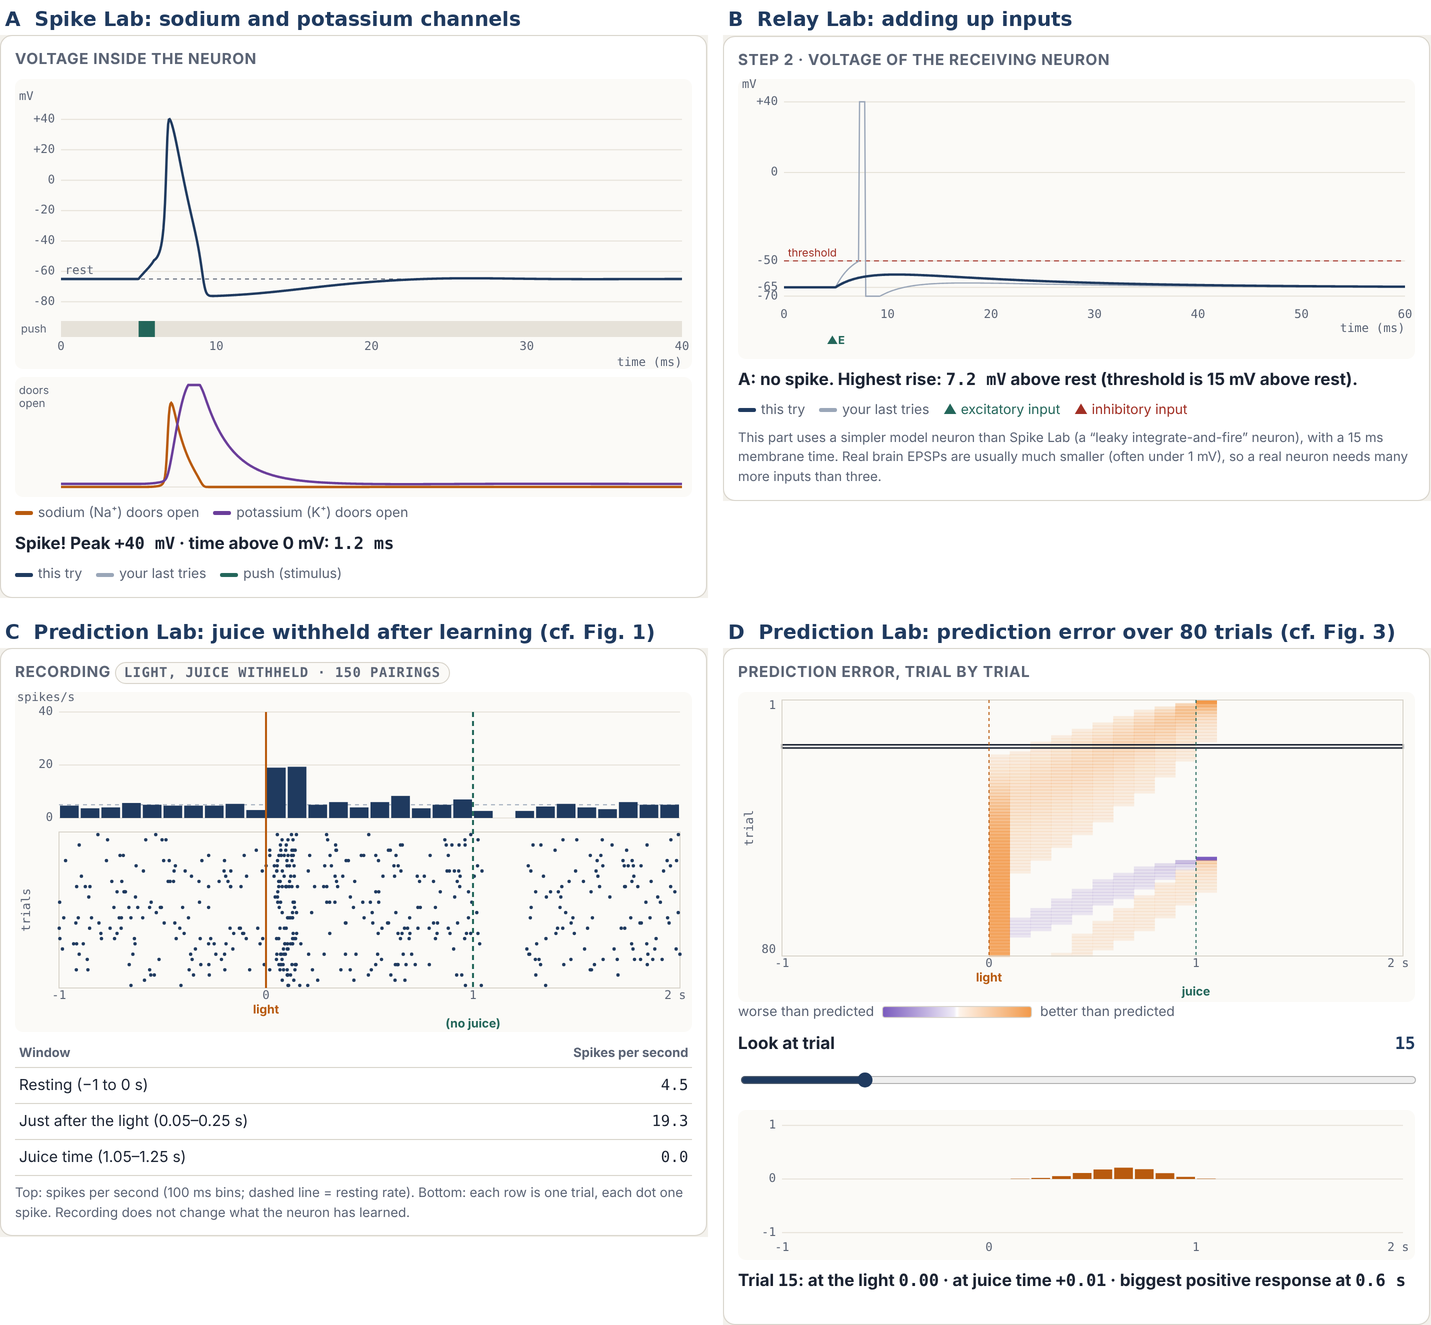
\includegraphics[width=0.92\linewidth]{figure1.png}
\caption{Four views from the labs. (A) Spike Lab: voltage, and sodium and potassium channel opening during a spike. (B) Relay Lab: one excitatory input stays below threshold; three together fire the cell (grey trace). (C) Prediction Lab: after training, a model dopamine neuron bursts after the light and pauses when the expected juice is withheld, as in Fig.~1 of \citet{schultz1997}. (D) Prediction error over 80 training trials moves from the juice back to the light, with a negative error on trial 50, when the juice was withheld, as in their Fig.~3.}
\label{fig:labs}
\end{figure}

\subsection{Learning objectives}

\paragraph{Spike Lab} (one 90-minute class). Students explain threshold and the all-or-none spike from their own measurements; describe the order of sodium and potassium channel opening and predict the effects of tetrodotoxin and tetraethylammonium; explain absolute and relative refractory periods and why spikes travel one way; and explain rate coding: stronger stimuli produce more spikes per second, not bigger spikes.

\paragraph{Relay Lab} (one 90-minute class covering three textbook sessions). Students explain why myelin, more than diameter, makes conduction fast and why demyelination slows it; order the steps of chemical transmission; distinguish spatial and temporal summation and the role of inhibition; and contrast ion-channel and G-protein receptors and classify drugs as agonists, antagonists or reuptake blockers.

\paragraph{Prediction Lab} (a 90-minute open-book assessment). Students read a raster plot and a peri-event histogram; state the reward-prediction-error account of dopamine neurons and test it against their own replication; connect a systems-level finding to spikes, synapses, conduction, receptors and drugs; and judge what a partial replication failure means for a theory.

% ---------------------------------------------------------------------
\section{Instructional design}

\paragraph{Predict, measure, record, check.} Every lab part follows the same cycle. Students predict, run the model, read a number from the screen and write it in their booklet. In the two teaching labs, numeric answers receive immediate, specific feedback (``a little low; check the readout'') rather than a red cross, multiple-choice questions explain the correct answer, and each part ends with a ``You are done when\ldots'' line so students know when to stop. A results page collects the student's numbers into one line to copy into the booklet.

\paragraph{Slides and lab together.} The slide decks use an ``at a glance'' format: a one-line summary at the top of every content slide, at most three points, a fixed colour for each ion, a ``today on one page'' picture at the start and end, and a short recap after each section. Lab moments are marked with a coloured tag and a QR code. Relay Lab locks each part until its slide shows a password, so that a class moves together; the passwords pace the class and are not a security measure.

\paragraph{Booklets.} Each lab part has its own booklet page with the time, who to work with, numbered steps and spaces for numbers. The activity booklets add a word list, study cards with short episodes from the history of neuroscience (Adrian's first single-fibre recordings, Eccles and Popper's ``soups versus sparks'' debate, the discovery of opiate receptors), worked answers and sources.

\paragraph{Accessibility.} The labs and materials were designed to be neurodivergent-friendly: one idea per screen, numbered steps, calm feedback, a typeface designed for legibility (Atkinson Hyperlegible), consistent colours, light and dark themes that follow the device, layouts that work at phone width, respect for the reduced-motion setting, keyboard access, and no sound unless the student turns it on.

\paragraph{Privacy and access.} The labs store and send nothing. They need only a browser; jsPsych is bundled, so a local copy runs without internet access. This makes the labs usable in classrooms with mixed devices and uneven connectivity, and means no student data needs to be managed.

\section{The read--replicate--explain assessment}

Prediction Lab and its question booklet form an assessment format designed to be reused with other papers. Students have 90 minutes and may use any course materials.

\begin{enumerate}
\item \textbf{Read} (10 marks, about 20 minutes). A one-page reading guide tells students which pages and figures to read closely and which to skim; the equations are explained in words. Questions ask students to interpret the rasters and histograms of the paper's Fig.~1, to classify each panel as a positive, zero or negative prediction error, and to explain why a well-timed pause with no external event implies an internal representation of time.
\item \textbf{Replicate} (15 marks, about 35 minutes). Students run the four lab parts and record their numbers: their own reaction times in the cue--reward task, recordings before and after learning, the trial numbers at which the response moves from reward to cue, and the responses to seven test conditions, each predicted before it is recorded.
\item \textbf{Connect} (10 marks, about 25 minutes). Five questions link the paper back to the course: how an all-or-none spike can signal ``worse than expected''; which synaptic inputs could produce a burst and a pause; how long a burst takes to travel along a thin unmyelinated axon; what G-protein-coupled dopamine receptors imply for timing; and why a reuptake blocker could make an experience seem better than expected every time.
\item \textbf{Think} (5 marks, about 10 minutes). Students choose one of three short arguments: whether a partial replication failure refutes the theory; whether dopamine is ``the pleasure chemical''; and who, if anyone, is ``surprised'' when a neuron signals a prediction error.
\end{enumerate}

Because simulated spikes are random, each student's numbers in the replication section differ slightly, which discourages copying while leaving the pattern unmistakable. The answer key and marking scheme are kept out of the public repository so the booklet can be reused, and are available to instructors on request.

A distinctive feature is a deliberate mismatch. With the temporal representation used in the paper's model (a ``complete serial compound''), juice delivered 0.5~s \emph{early} produces a burst at the early time \emph{and} a pause at the usual time. The paper's own note 18 reports that real neurons paused at the usual time only when the reward was late \citep[see also][]{hollerman1998}. The lab keeps this behaviour, and one of the ``Think'' questions asks students to find the discrepancy and decide whether it falsifies the prediction-error account or only one modelling assumption. Students thus experience a replication that partly fails, and reason about what follows.

% ---------------------------------------------------------------------
\section{Models and validation}

Every simplification is stated in the lab, the slides' speaker notes or the booklet, and documented in the repository's model notes.

\paragraph{Spike Lab} integrates the Hodgkin--Huxley equations for the squid giant axon at 6.3\,\textdegree{}C, resting near $-65$~mV, with forward Euler steps of 0.01~ms. Stimulus strength is a 0--10 classroom scale (1~ms pulses in Parts 1--3, a 200~ms step in Part 4). The potassium blocker removes 90\% of the voltage-dependent potassium conductance but keeps its resting part, so the cell still rests at $-65$~mV; blocking all of it makes the model fire spontaneously, which would obscure the lesson. Students are told that a cold squid axon has longer refractory periods than a warm mammalian neuron.

\paragraph{Relay Lab.} Part 1 is not a simulation: conduction speed follows empirical rules of thumb, about 6~m/s per micrometre of diameter for myelinated mammalian fibres \citep{hursh1939} and about $\sqrt{d}$~m/s for unmyelinated fibres of diameter $d$~\textmu m. Part 2 uses a leaky integrate-and-fire neuron with conductance-based synapses and a 15~ms membrane time constant. The Hodgkin--Huxley neuron was tried first but summed inputs only over 2--3~ms, too short to show temporal summation over the 1--15~ms range that textbooks describe. Each excitatory input here depolarises the cell by about 7~mV, much more than a typical cortical EPSP, and the lab says so. Part 3 uses simplified receptor kinetics in arbitrary units; only the direction of each drug's effect is meant literally.

\paragraph{Prediction Lab} implements the paper's temporal-difference rule (its Eqs.~3--5): each light is represented by a chain of signals, one per 100~ms step after onset, each with its own weight; the prediction error is $\delta(t) = r(t) + \gamma V(t+1) - V(t)$, with $\gamma = 0.98$ and learning rate $\alpha = 0.3$, applied once per trial. The error drives a Poisson spike generator with a resting rate of 5 spikes/s, within the 0.5--7 spikes/s reported for monkey dopamine neurons \citep{ljungberg1992}; positive errors add a 100~ms burst and negative errors a 200~ms pause, both starting 50~ms after the event, close to the reported burst latency \citep{schultzromo1990}. These display settings are choices, not fits to data. The ``receptor blocker'' halves the learning rate, following the paper's point that animals given dopamine receptor blockers learn more slowly.

\paragraph{Validation.} An end-to-end test suite serves the site, opens each lab in a headless browser at laptop and phone sizes, works through every part as a student would, and checks 96 conditions, including that each value the booklets rely on is produced (Table~\ref{tab:checks}), that wrong passwords are refused, that no page scrolls sideways at phone width and that no browser errors occur. The tests run on every commit through continuous integration.

\begin{table}[ht]
\centering\small
\caption{Values checked by the automated tests. Prediction Lab rates vary slightly between recordings; its trial numbers are exact.}
\label{tab:checks}
\begin{tabularx}{\linewidth}{@{}>{\raggedright\arraybackslash}p{2.2cm}>{\raggedright\arraybackslash}X>{\raggedright\arraybackslash}p{5.2cm}@{}}
\toprule
Lab & Measurement & Value\\
\midrule
Spike Lab & weakest strength that fires & 4.5 (4.0 does not)\\
 & peak at threshold; at strength 10 & about $+37$~mV; $+41$~mV\\
 & time above 0~mV: normal; potassium blocker & 1.2~ms; 2.6~ms\\
 & shortest gap for two spikes at strength 8; 10 & 13~ms; 12~ms\\
 & firing rate at strengths 1, 3, 5, 7, 10 & 5, 80, 90, 105, 115 spikes/s\\
\addlinespace
Relay Lab & speed: 1~\textmu m bare; 12~\textmu m myelinated; squid; 12~\textmu m demyelinated patch & 1; 72; 22; 10 m/s\\
 & inputs needed to fire; longest effective gap for one repeated input & 3 together; 7~ms\\
 & peak with antagonist; with clearance blocker (no drug = 100) & 15; about 210 (ion channel), about 290 (G-protein)\\
\addlinespace
Prediction Lab & reward response below half; transfer to the cue & trial 3; trial 26 (blocker: 6; 49)\\
 & after training: light; juice; juice withheld & about 17; 5; 0 spikes/s\\
 & light 2 omitted: at 0.5~s; at 1.0~s & pause; smaller burst\\
\bottomrule
\end{tabularx}
\end{table}

% ---------------------------------------------------------------------
\section{Classroom use}

The module was developed for PSYC343 \emph{Introduction to Neuroscience}, an undergraduate psychology course at Krea University, India, taught from \citet{bear2016}. It grew out of feedback from a teaching assistant after a class on membrane potentials: the slides were hard to follow at a glance, and students struggled to keep up. Rewriting the decks in an at-a-glance format raised a further question, whether students could \emph{do} each idea beside the slide rather than only watch it. Spike Lab came first. Relay Lab followed when the syllabus had to be shortened and three textbook sessions were combined into one class. Prediction Lab began as the course's second quiz and became a rehearsal for the end-term examination, which uses the same read--replicate--explain format with a different paper.

All three labs, with their slides and booklets, were introduced in class to a cohort of 45 undergraduate students in 2026. In class, students said that they enjoyed the lab sessions. No data were collected from students, so this is an informal impression rather than evidence of learning; a formal evaluation is planned (Section~\ref{sec:limits}).

% ---------------------------------------------------------------------
\section{Limitations and planned evaluation}\label{sec:limits}

The labs have not yet been evaluated for learning gains. The models are deliberately simplified: Spike Lab is a cold invertebrate axon; Relay Lab's conduction speeds are rules of thumb, its EPSPs are larger than real ones and its receptor kinetics are qualitative; Prediction Lab's neuron is a display of a learning rule, not a fitted model of dopamine cell physiology. The assessment format depends on students being able to read a primary paper in English within the time allowed, which the reading guide supports but does not guarantee. Finally, the pacing passwords and the start password can be found by anyone who reads the page source; they organise a class but do not secure an examination.

A planned evaluation, subject to institutional ethics approval, will compare concept-inventory scores before and after each lab class, analyse performance on the assessment's sections, and survey students on usability and accessibility. Reports from other instructors who adopt the labs are invited through the repository's issue tracker.

\section{Availability and adaptation}

The module is available at \repo{} and runs at \site. Code is released under the MIT licence; booklets, slides, documentation and figures under CC BY 4.0. The repository includes an instructor guide (learning objectives, timings, pacing passwords, the assessment format and how to adapt everything), model notes, contribution guidelines and the test suite. Slides and booklets are LaTeX sources; changing one link per file updates every QR code. Instructors can fork the repository and serve their own copy with GitHub Pages or any web server.

\section*{Declarations}

\paragraph{Use of generative AI.} Claude (Anthropic), a generative AI model, was used to assist with checking and debugging the lab code. The author reviewed all changes and takes full responsibility for the code and materials.

\paragraph{Ethics.} No data were collected from students for this article, so ethics approval was not required. The classroom-use section reports only the author's informal observations. The labs themselves store and send no data.

\paragraph{Funding.} This work received no specific funding.

\paragraph{Competing interests.} The author declares no competing interests.

\paragraph{Acknowledgements.} I thank the teaching assistants of PSYC343, Judith Grace Lazarus and Namrita Thakur, for their feedback on the slides and labs, and the students of the course for their enthusiasm.

\bibliographystyle{apalike}
\bibliography{references}

\end{document}
